\chapter{Versuch 1}

\section{Benötigte Geräte}

Für dieses Experiment benötigen wir die Folgenden Geräte:


\begin{table}[h]	
	\centering
	\begin{tabular}[h]{c|c|c}
		\centering
		Gerät & Anzahl & Produktbeeichnung\\
		\hline
		Oszilloskop & 1  & Keysight DSOX1102A\\
		\hline
		% Frequenzgenerator & 1 & TELEDYNE T3AFG80\\
		% \hline 
		Digital-Multimeter & 1 & Fluke 87V TRUE RMS MULTIMETER\\
		\hline 
		Widerstand 1k$\Omega$ & 9 &  \\
		\hline 
		Widerstand 10k$\Omega$ & 1 &  \\
		\hline
		LED & 8 & \\
		\hline
		ADC & 1 & ADC0804LCN \\
		\hline
		Kondesator 0,1 $\mu$F & 2 & \\
		\hline
		Kondesator 10 $\mu$F & 1 & \\
		\hline
		Kondesator 150 pF & 1 & 
			\label{tab:Materialliste Versuch 1}
	\end{tabular}
	\caption{Materialliste Versuch 1}
	\label{tab:Materialliste Versuch 1}
\end{table}

\section{Versuchsaufbau}


\begin{figure}[H]
	\centering
	\includegraphics[height=10cm]{images/Schaltskizze_versuch1.pdf} 
	\caption{Schaltungsskizze}
	\label{fig: Schaltungsskizze}
\end{figure}

Zunächst einmal die Schlatungsskizze (Abbildung \ref{fig: Schaltungsskizze}) für unseren Versuchsaufbau.

Aufgrund des Fehlen des Schalters haben wir diesen durch ein Kabel ersetzt, welches 
durch einstecken in das Steckbord den Schalter simuliert. \par

Man geht zunächst einmal davon aus, dass die Clockfrequenz des ADC 600 kHz beträgt.\par
Bei der Verschaltung sollte man beachten, dass die Eingangspins 1 - 5, 10, 19 und 20 
haben digitale Referenzwerte, wobei die Eingangspins 6 - 9 - analoge.\par
Der V(+)-Eingang muss mit einem Schutzwiderstand 1 k\textOmega  gegen Überspannungen 
und mit einem 0.1 \textmu F gegen Einstreuungen versehen werden. \par

Die Betriebs- und Eingangsspannungen werden mit Hilfe des \acs{DMM} gemessen, um sie möglichst 
genau zu bestimmen.\par
Das Bitmuster wird von den \acs{LED}s in binärer Darstellung abgelesen. Ein \acs{LSB} beträgt 20 mV.\par
Die Versorgungsspannung für den Versuch liege bei 5,120V. Diese definiert den 
Eingangsspannungsbereich U\textsubscript{in}: 0 bis 5,120V. \newline


Die Schaltung wurde aufgebaut und von einem Betreuer überprüft. Danach wird die Schaltung
mit V\textsubscript{dc} ca. 5,133V in Betrieb genommen. \par

\begin{figure}[H]
	\centering
	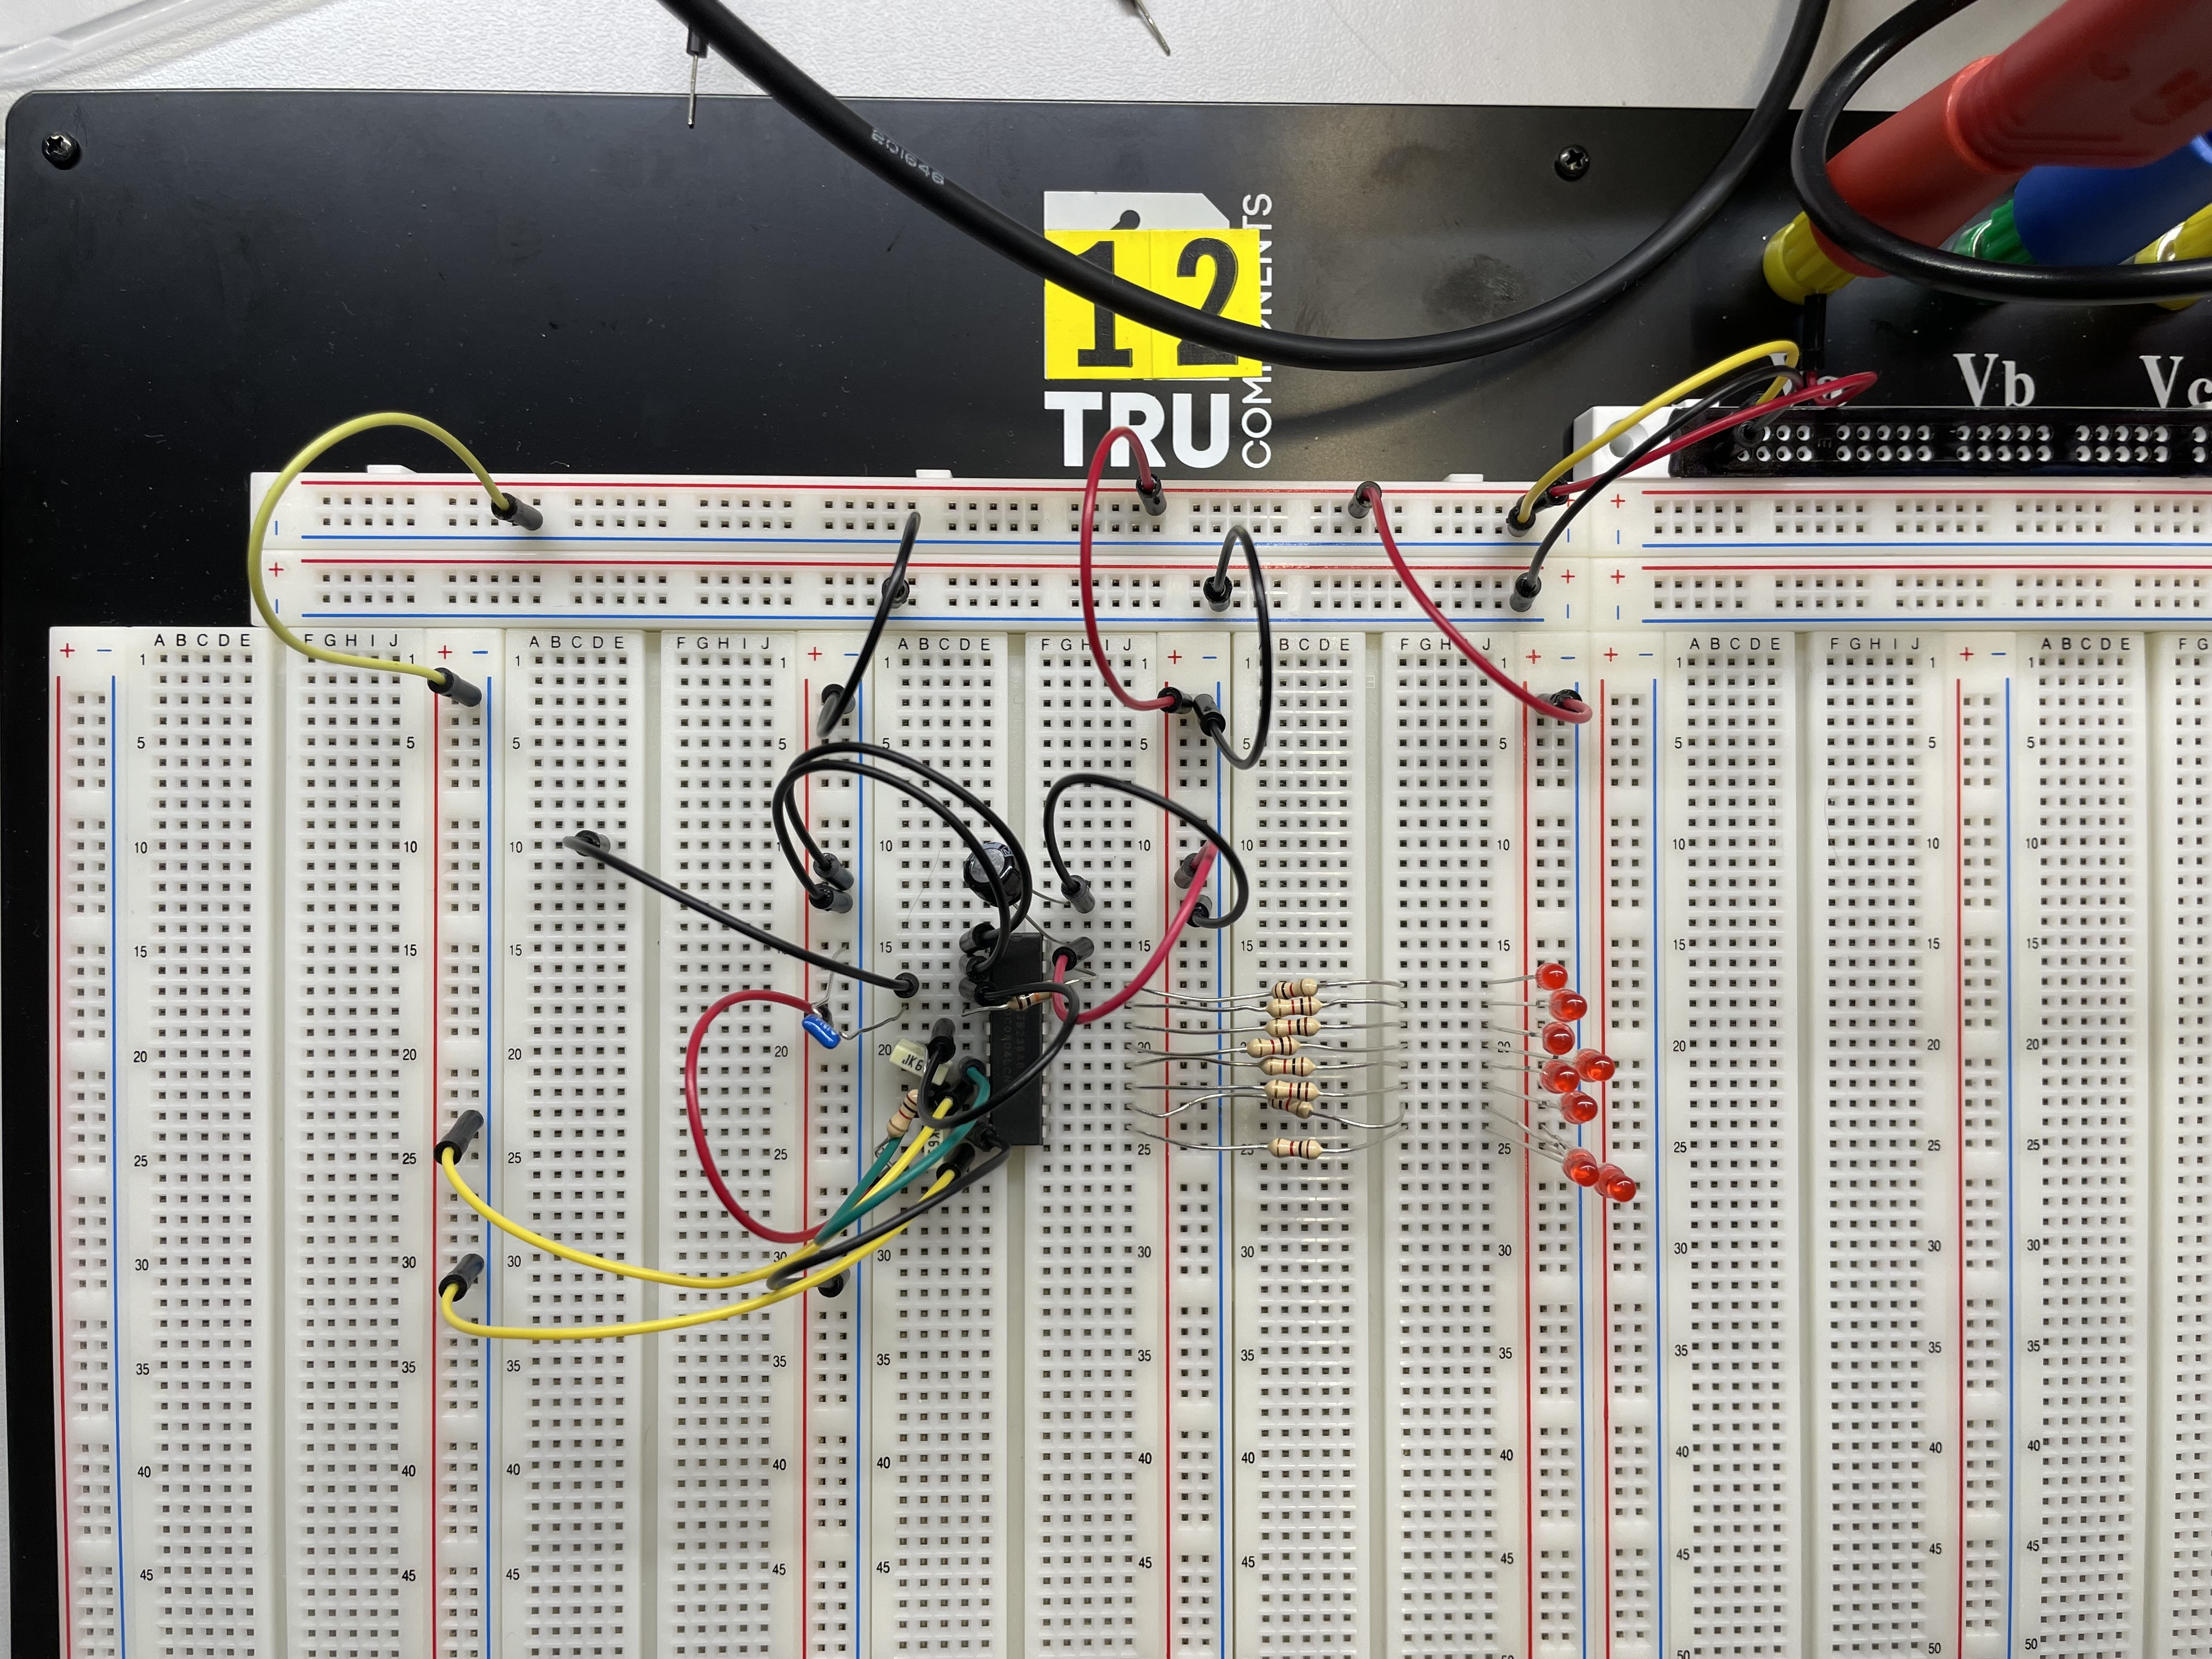
\includegraphics[height=7cm]{images/Schaltungsaufbau-versuch-eins.jpeg} 
	\caption{Schaltungsaufbau}
	\label{fig: Schaltungsaufbau}
\end{figure}

Der digitale Output der Schaltung wird von den \acs{LED}s in Abbildung 
\ref{fig: Schaltungsaufbau} dargestellt.
Bei der Inbetriebnahme wurde festgestellt, dass die Signale invertiert sind, 
und der Zustand An einer Null entspricht, der Zustand Aus - einer Eins.

\section{Integrale Nichtlinearität}

In disem Abschnitt soll die Integrale Nichtlinearität in dem gesamten Bereich gemessen
werde. Dafür soll die Eingangsspannung in 16 gleich große Bereiche unterteilt werden, was 
320mV Stufen ergibt. Man fährt jeweils die Breichsgrenze von unten an und protokolliert 
die für den Bitsprung notwendige Eingangsspannung in einer Tabelle.


\begin{table}[H]
	\centering
	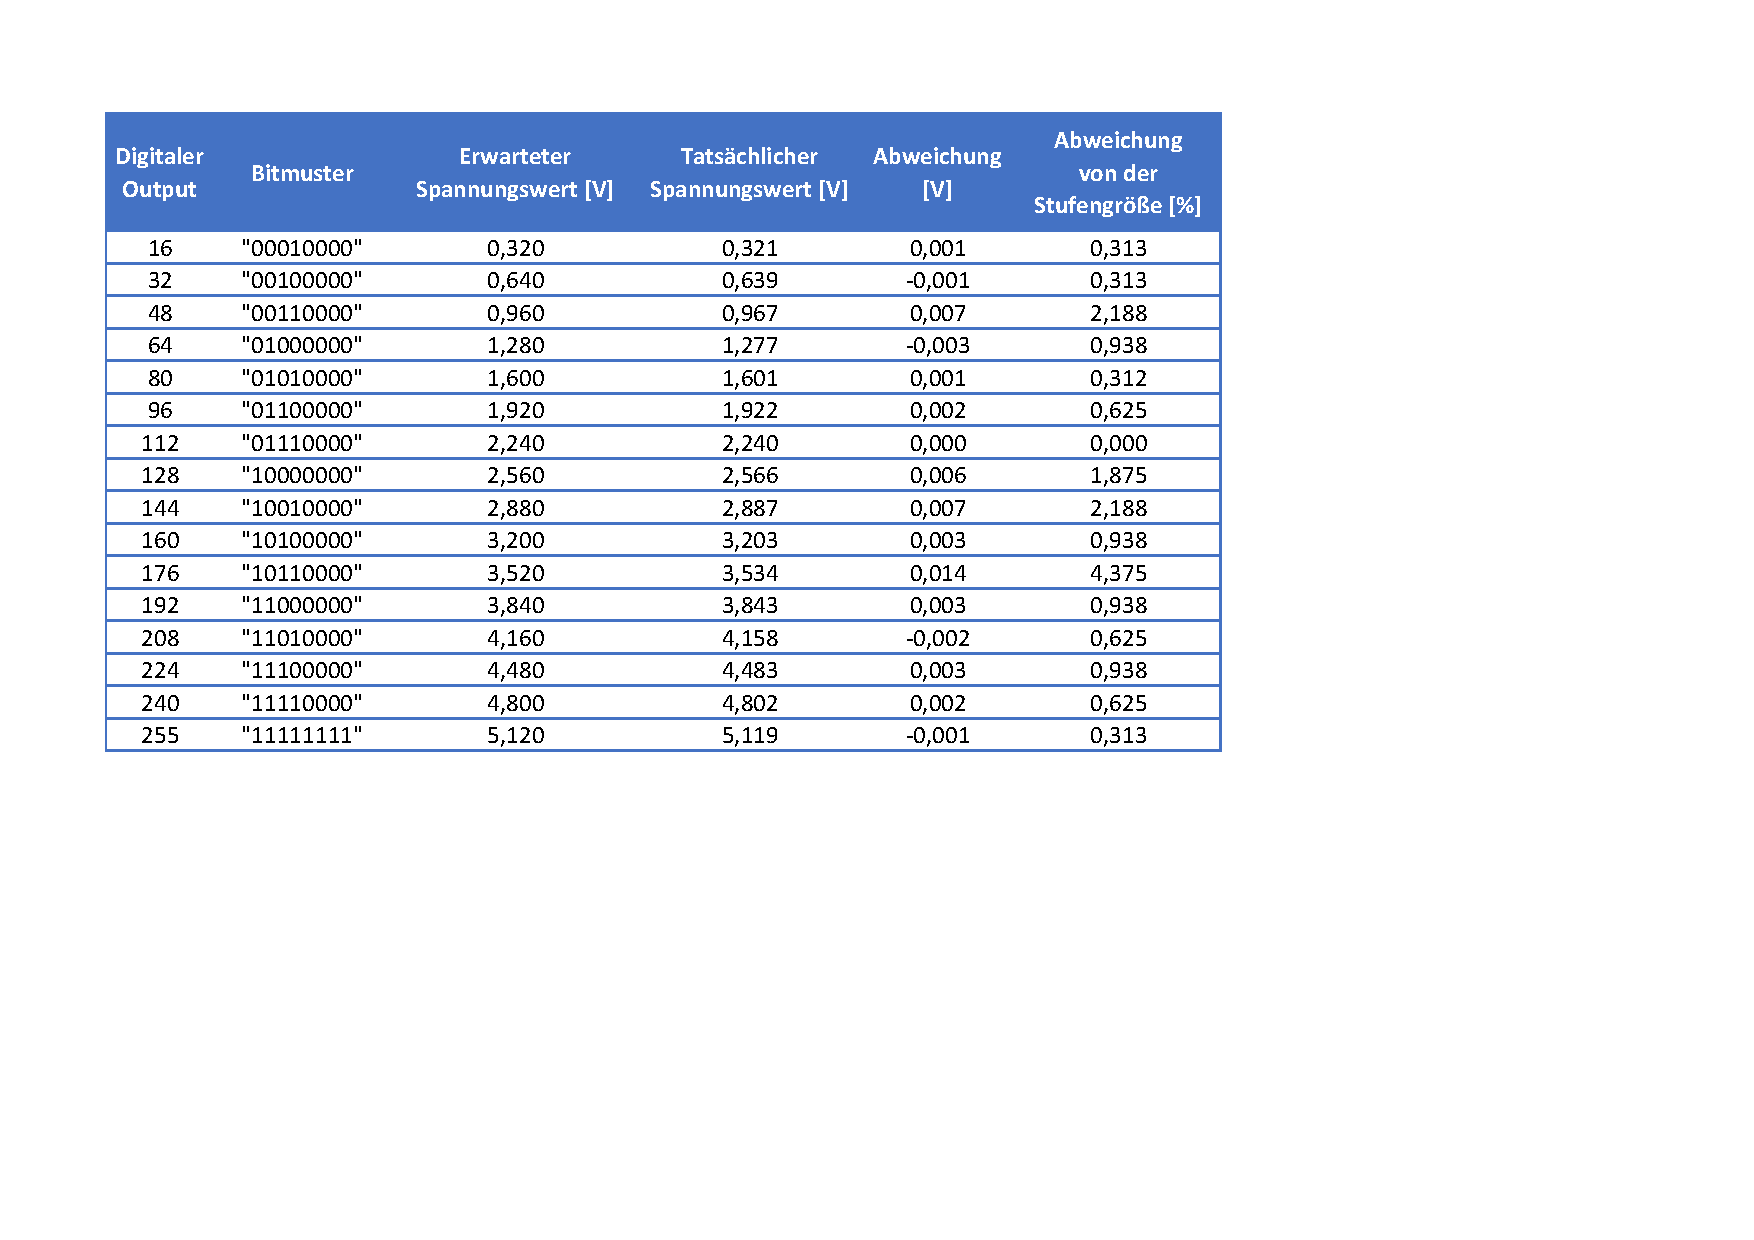
\includegraphics[height=7cm]{images/Versuch1d.pdf} 
	\caption{Ergebnisse Integrale Nichtlinearität}
	\label{fig: Ergebnisse Integrale Nichtlinearität}
\end{table}

Anhand der erwarteten und tatsächlichen Werte wird die Abweichung in V und Prozent
berechnet. Die größte Abweichung von der Idealgeraden beträgt lediglich 14 mV, 
was ca. 4.375\% der Stufengröße entspricht. \par

Man stellt diese Werte als zwei Geraden in einem Graphen.

\begin{figure}[H]
	\centering
	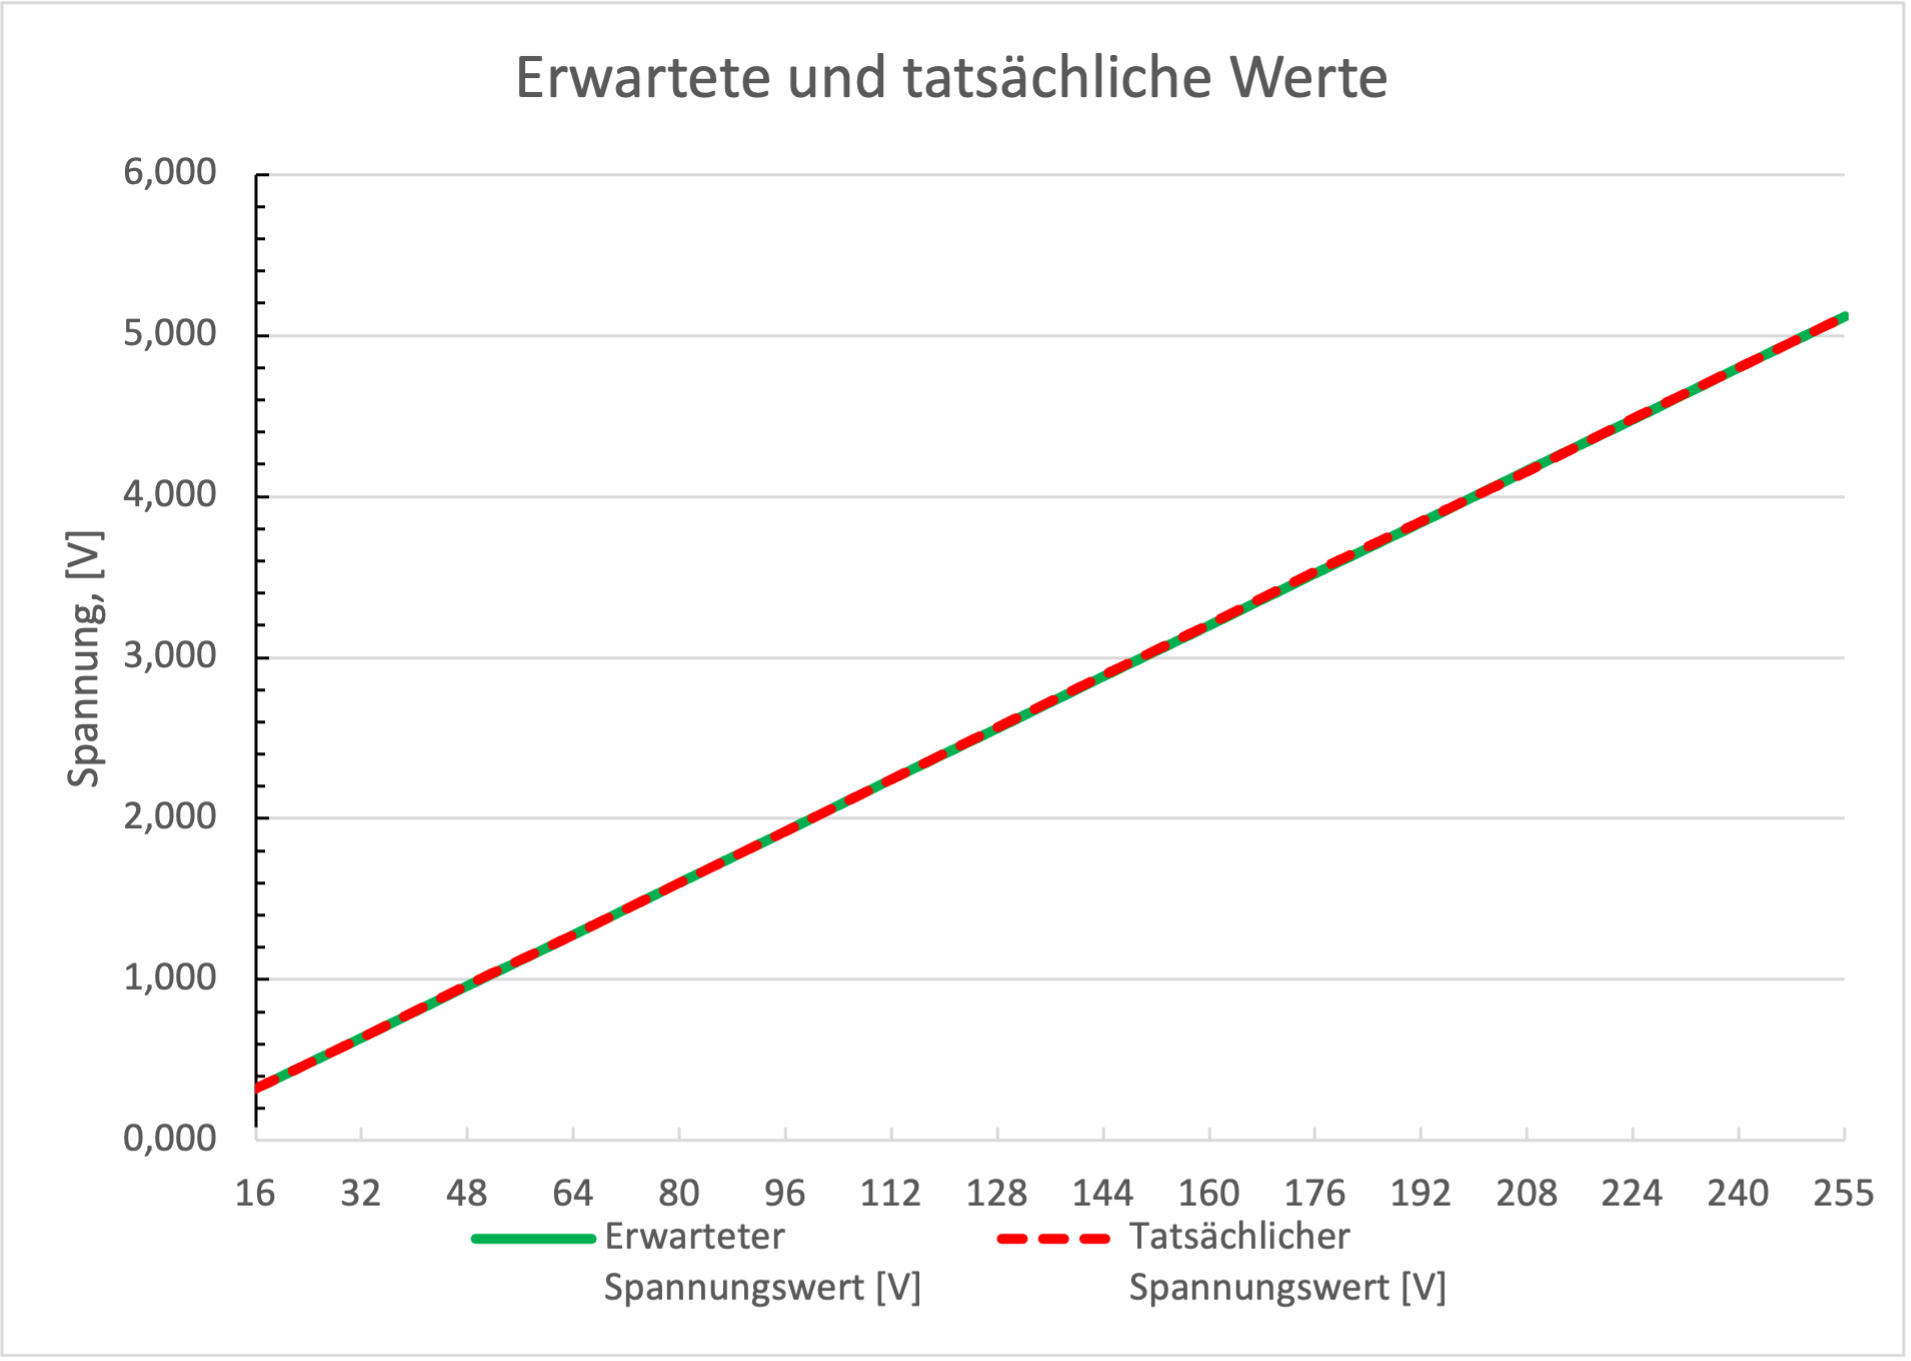
\includegraphics[height=7cm]{images/INL_gerade.png} 
	\caption{INL erwartete und tatsächliche Werte}
	\label{fig: INL erwartete und tatsächliche Werte}
\end{figure}

Es ist deutlich sichtbar, dass die Geraden nahezu identisch verlaufen.\par

Als nächstes, stellt man die Abweichungen als Histogramm dar. 

\begin{figure}[H]
	\centering
	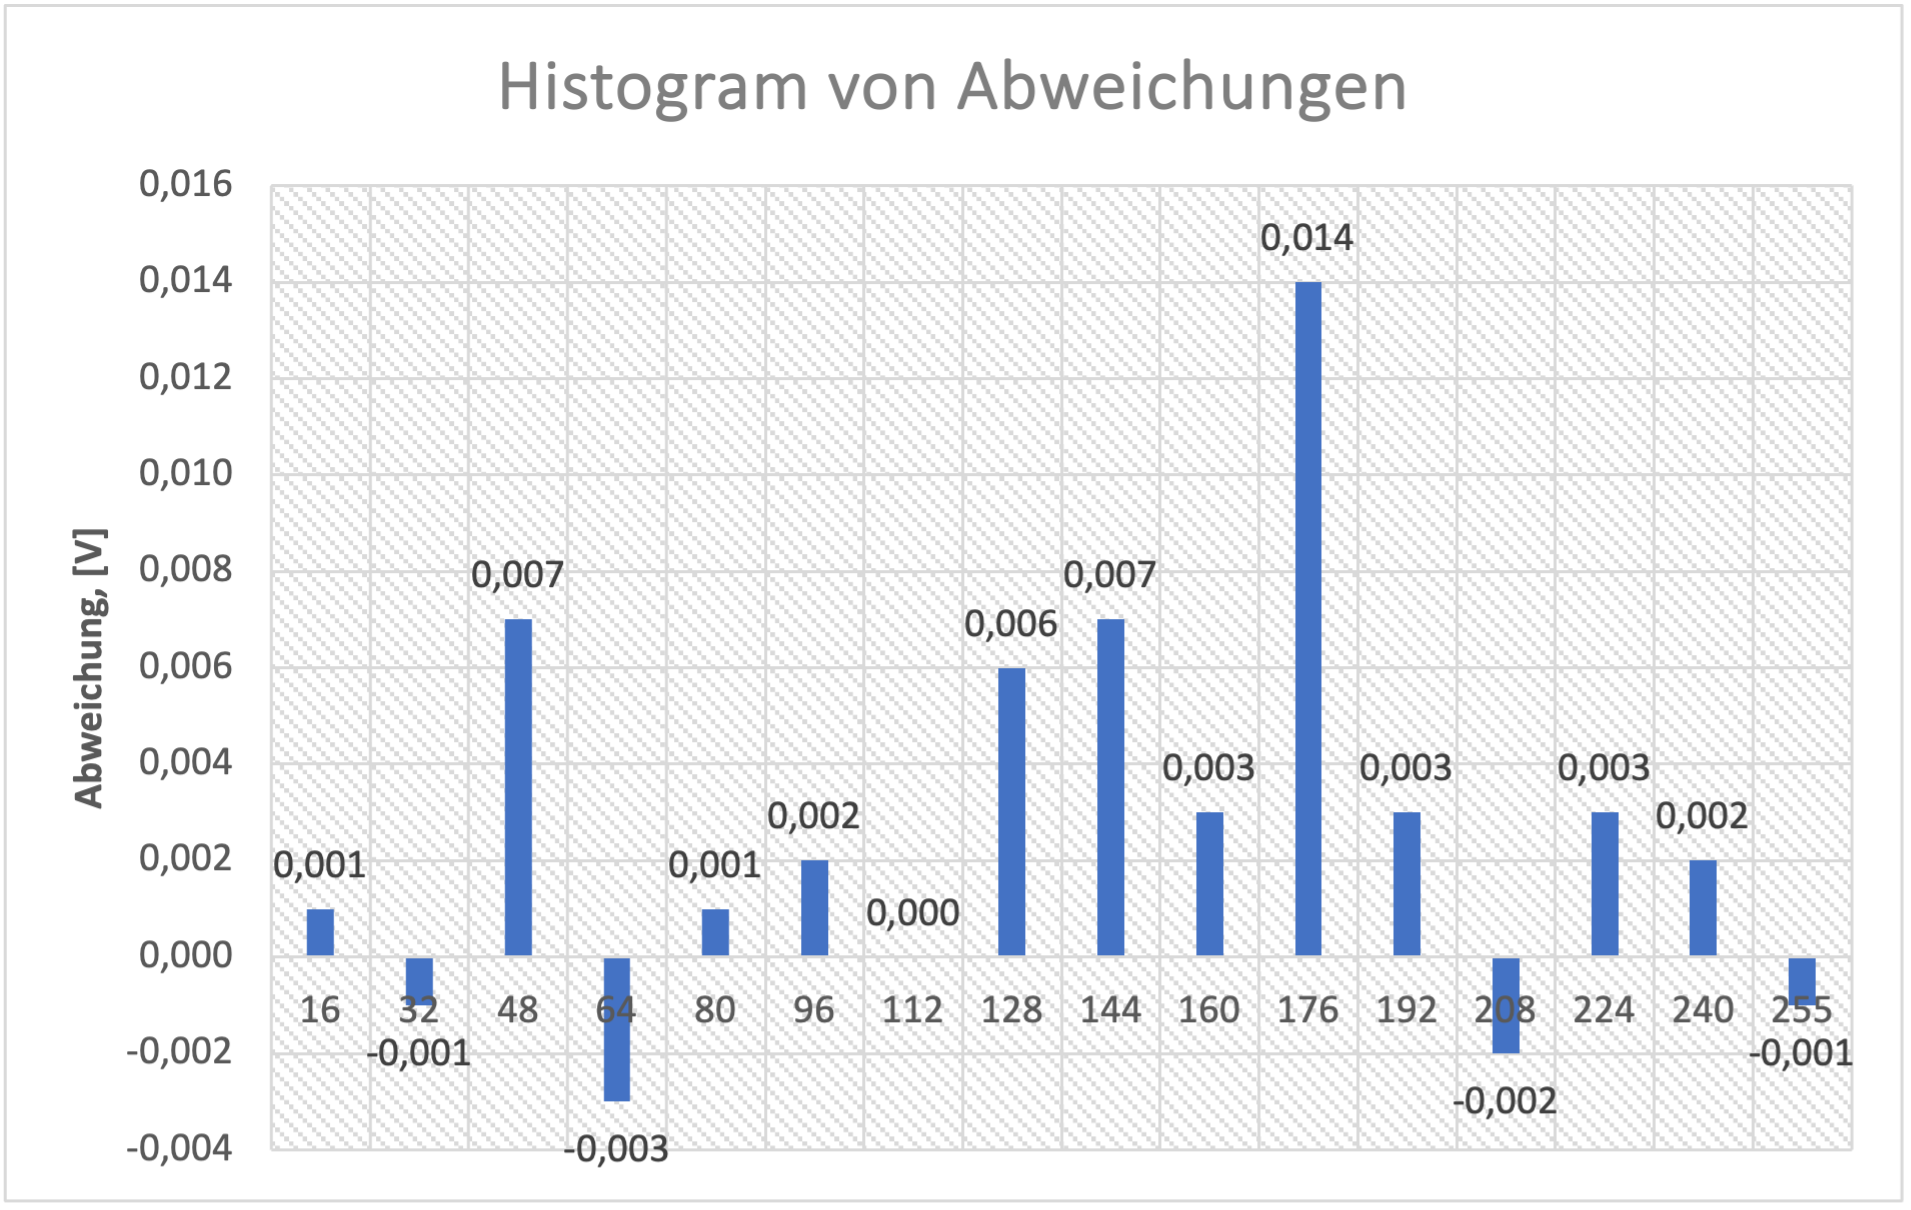
\includegraphics[height=7cm]{images/Histogramm_versuch1.png} 
	\caption{INL Verteilung der Abweichungen von der
	Idealgeraden als Histogramme}
	\label{fig: INL Verteilung der Abweichungen von der
	Idealgeraden als Histogramme}
\end{figure}

Das Mittelwert der Abweichung beträgt 3,5mV, was die Qualität und Genauigkeit
des ADCs und allgemein des Verfahrens SAR zeigt.
Die Spitze in Höhe von 14mV bei dem Digitalen Output 176 lässt sich vermutlich 
dadurch erklären, dass die Einstellung von dem Input an dem Netzgerät über keine 
Feinfunktion verfügt (Ungenauigkeit der Messung).

\section{Differentiale Nichtlinearität}
In diesem Abschnitt wird die Differentiale Nichtlinearität von dem ADC gemessen.
Man misst die neun um die Bereichsmitte liegende Werte, die jeweils ein LSB Abstand
voneinander haben. Das Verfahren bleibt gleich: man fährt jeweils die Breichsgrenze 
von unten an und protokolliert die für den Bitsprung notwendige Eingangsspannung in 
einer Tabelle. Außerdem berechnet man die jeweilige Differentiale Nichtlinearität und
trägt entsprechend in die Tabelle ein.

Die DNL lässt sich mit der Formel 
\[
\text{DNL} = \frac{U\textsubscript{x+1} - U\textsubscript{x}}{U\textsubscript{LSB}} - 1
\]
berechnen. DNL darf den Wert von ± 1 nicht überschreiten, sonst kann es zu 
Monotonieverletzung und/oder missing codes führen. Die unten dargestellte Tabelle
zeigt die protokollierten Werte sowie die berechnete DNL.

\begin{table}[H]
	\centering
	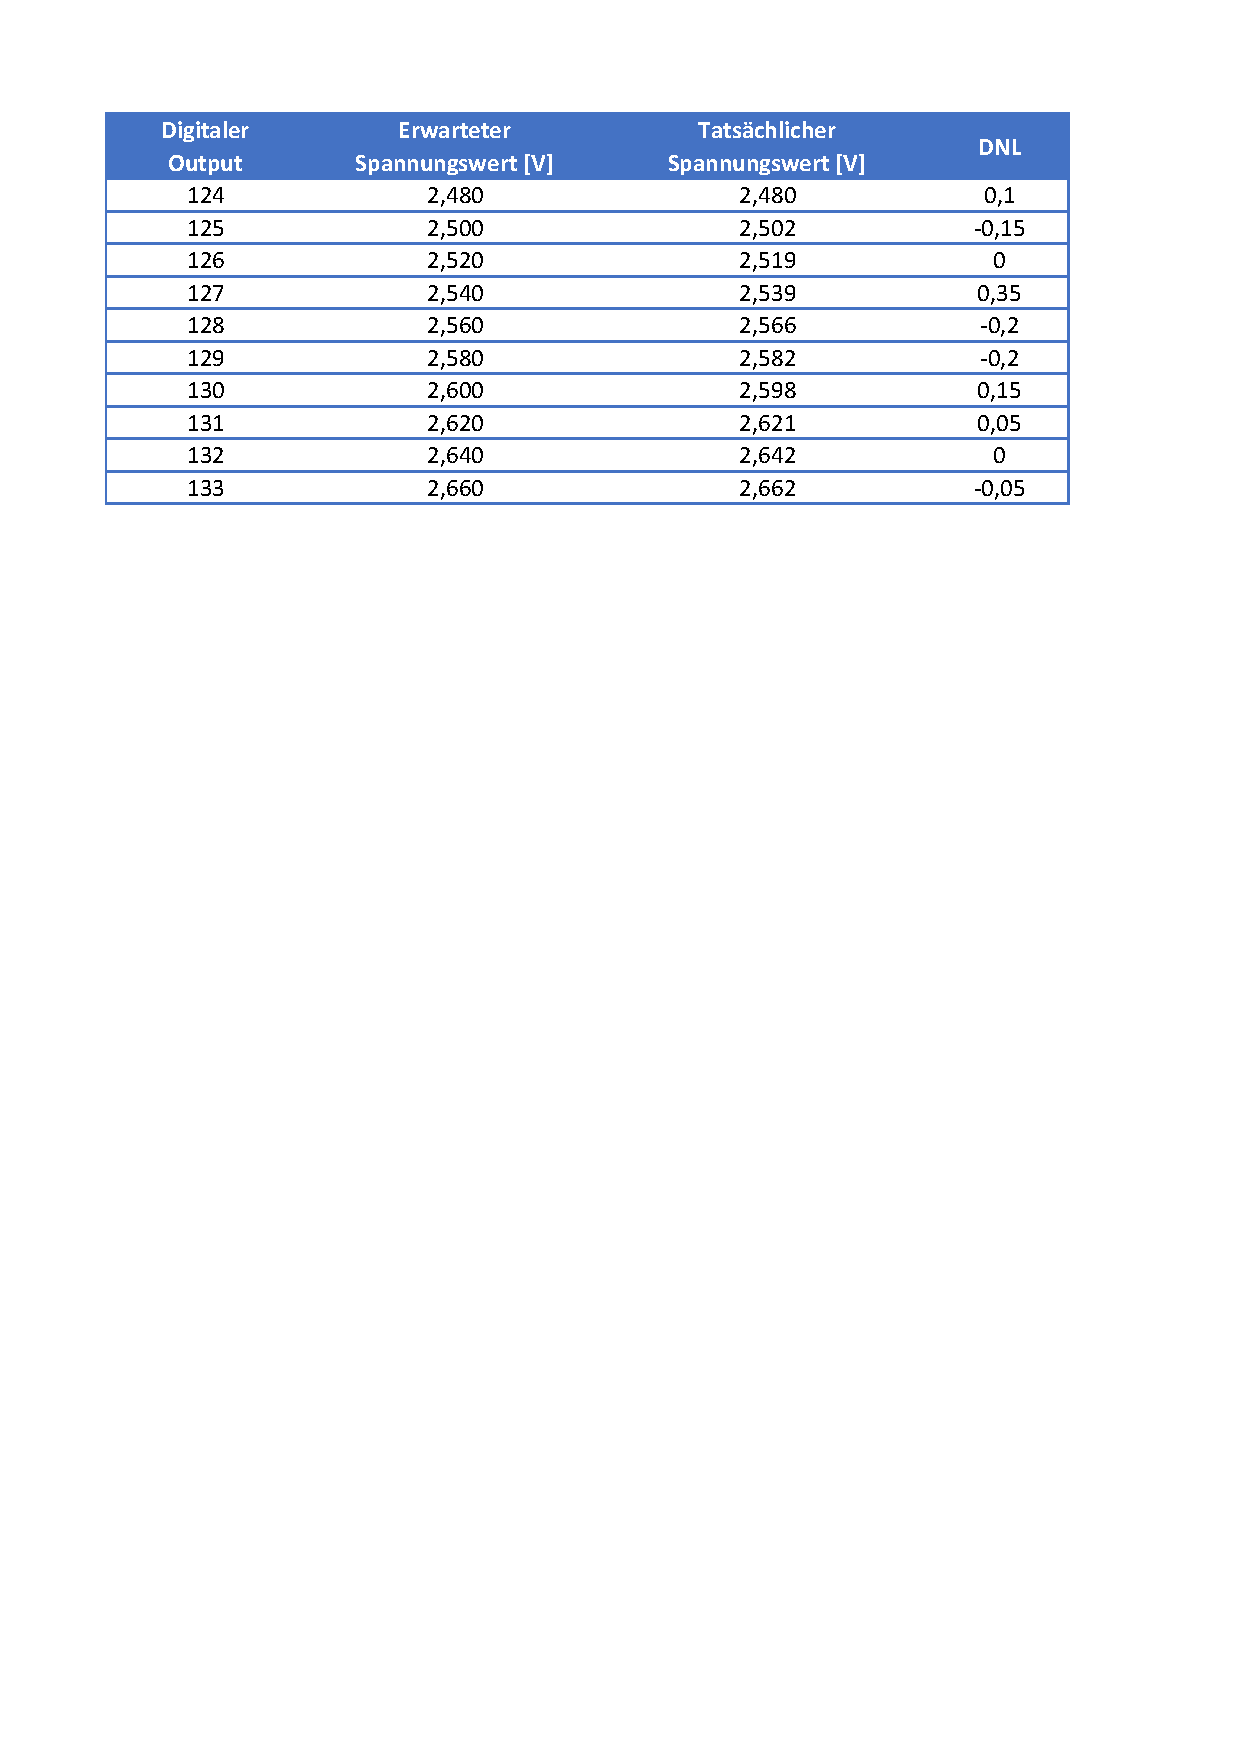
\includegraphics[height=7cm]{images/DNL_Tabelle.pdf} 
	\caption{DNL}
	\label{table: DNL}
\end{table}

Anhand der Daten lässt sich ein Graph bilden, wo die tatsächliche und erwartete
Werten in der Form einer Treppenfunktion dargestellt sind. Außerdem sind auf dem
Graphen die ideale und tatsächliche Geraden (gehen durch den Ursprung und durch die
Mitten der Treppenfunktion) aufgetragen.

\begin{figure}[H]
	\centering
	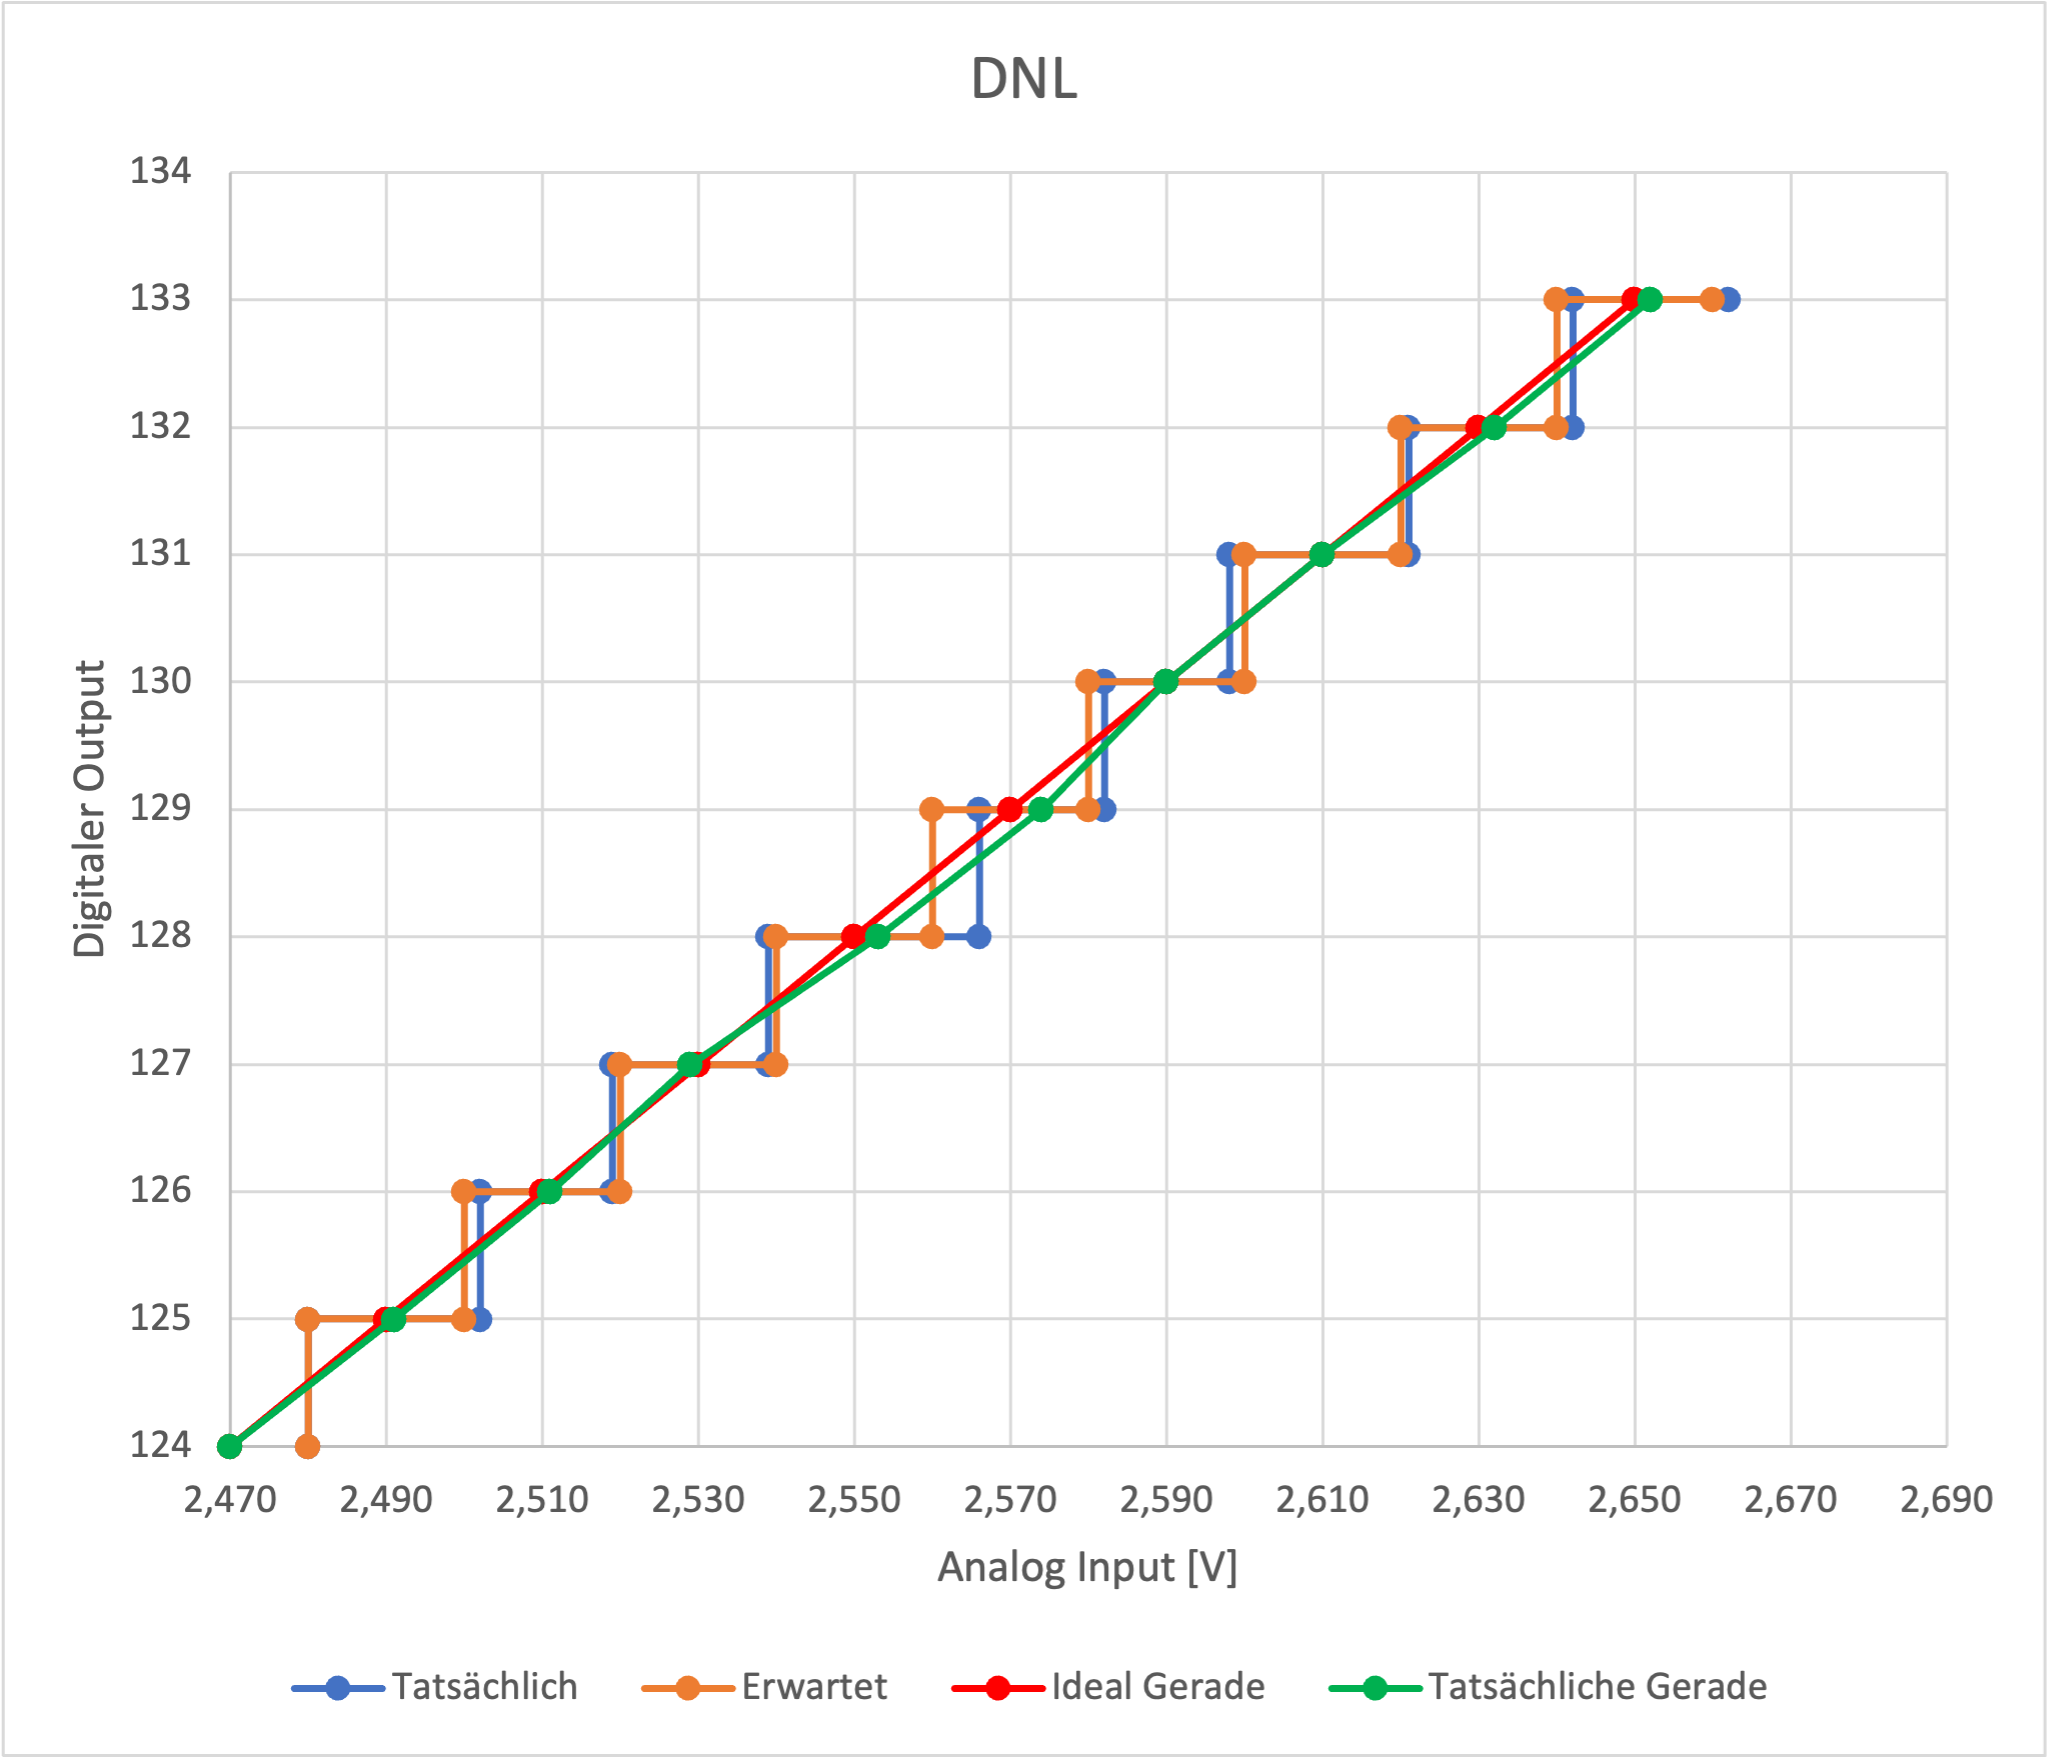
\includegraphics[height=11.5cm]{images/DNL.png} 
	\caption{DNL}
	\label{fig: DNL}
\end{figure}

Aus diesem Graphen lässt sich folgendes Verhalten ablesen: die Geraden und die
Treppen verlaufen hier gleicherweise nahezu identisch, allerdings es ist sichtbar,
dass es bei den Digitalwerten 128 und 129 deutliche Abweichungen gibt.

\section{Konversionszeit}
In diesem Abschnitt wird die Konversionszeit gemessen. Dafür wird Oszilloskop
wie in Abbildung \ref{fig: Clock Intervall} eingestellt.

\begin{figure}[H]
	\centering
	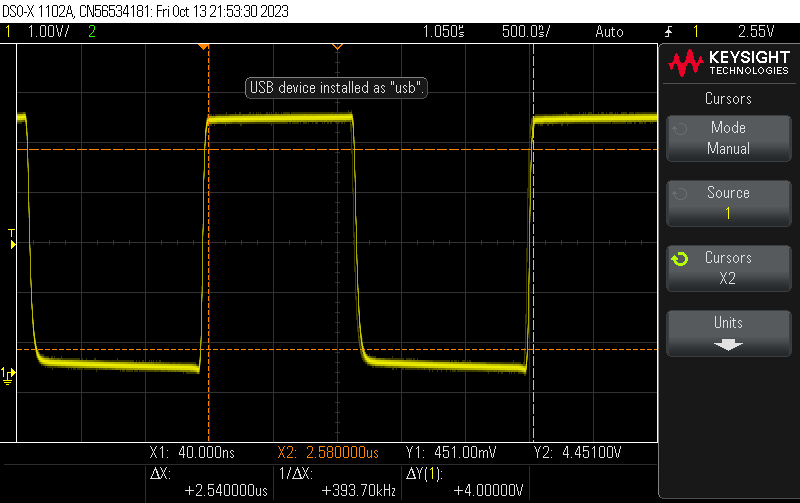
\includegraphics[height=7cm]{images/Clock-interval.png} 
	\caption{Clock Intervall}
	\label{fig: Clock Intervall}
\end{figure}

Durch das Einstellen der Cursor kann die Zykluszeit abgelesen werden: 2,54$\mu$S.
Daraus wird die Frequenz berechnet bzw. auch abgelesen ($\text{f\textsubscript{CLK}}=\frac{1}{t}$): 
393,70kHz.\par

Folgende Abbildung zeigt die Konversionszeit (die Zeit, die für eine Konversion
eines Digitalwertes in einen Analogwert gebraucht wird).

\begin{figure}[H]
	\centering
	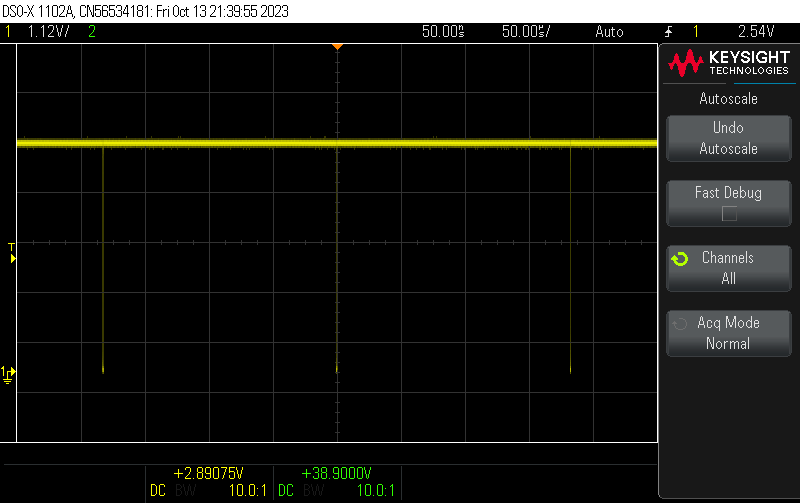
\includegraphics[height=7cm]{images/Conversion-Time.png} 
	\caption{Konversionszeit}
	\label{fig: Konversionszeit}
\end{figure}

Abgelesen mit Cursor (in der Abbildung leider nicht dargestellt) beträgt
die Konversionszeit 181,2$\mu$S. Die typische Konversionszeit laut dem Datenblatt
hat den Wert zwischen 103 und 114$\mu$S. Diese ist aber in Bezug auf die Clockfrequenz
f\textsubscript{CLK}=640kHz definiert. Die im Versuch gemessene f\textsubscript{CLK}
hat den Wert 393,70kHz, wodurch dieser Unterschied entsteht.\par

Weiter wird berechnet, wie viele Clock-Zyklen werden für eine Konversion benötigt.
Dies lässt sich mit einfacher Formel
$\text{T\textsubscript{C}}=\frac{t\textsubscript{konv}}{t\textsubscript{CLK}}$
berechnen. Die T\textsubscript{C} beträgt 
$\text{T\textsubscript{C}}=\frac{181.2\mu S}{2.54\mu S}=71.33\frac{1}{f\textsubscript{CLK}}$.
Vergliechen mit dem Datenblatt, liegt dieser Wert innerhalb des im Datenblatt
angegeben Intervall (zwischen 66 $\frac{1}{f\textsubscript{CLK}}$ und 73 $\frac{1}{f\textsubscript{CLK}}$).
